\section{Visualization}
\label{sec:vis}

The novelty of this work is pictured through the 3-dimensional visualization. The visualization is comprised of multiple layers where there is a natural visual connection between the layers. Many different methods could represent this data correlation however, we have created a novel visualization where the weather above affects the people below. The layers are connected via line bundles to dictate how the majority of the Twitter users in Nebraska are feeling.

\subsection{Layers}
The visualization is represented by three main layers. The base layer contains the map of Nebraska and neighboring states. We have chosen to show the counties in Nebraska to gain insight on the population distribution in the state, however we choose to keep the other states plain to indicate emphasis of correlation to Nebraska as shown in Figure \ref{fig:blur}.

On the map of Nebraska, there are red circles which indicate the area that Twitter users are posting from. The radius of the circle corresponds to the amount of people posting tweets in the vicinity. Using the WRF data set for the longitude and latitude values for the map, we obtained the intermediate values via interpolation. For each tweet location, the euclidean distance is calculated to get the nearest longitude and latitude location.

The middle region contains the line bundles which starts from the Twitter user location and ends at the weather cluster they correspond to above depending on the sentiment. The topmost layer is the weather clusters.

The middle region contains the line bundles from the Twitter user location to the weather cluster they correspond to above depending on the sentiment.The topmost layer is the weather clusters.


\subsection{Cloud Reperesentation}
Each cluster is represented by a different color. Clusters which aren't connected of the same color indicate the same conditions such as similar temperature, in other locations of Nebraska as seen in Figure \ref{fig:blur}.

Once the cluster for each hour was attained we needed two edge points for the data to link up to. These two edge points correspond to positive and negative emotions. We had different ideas on how the points should be picked. At first we were thinking to give half of one cluster to the positive emotion and the other half to negative emotions. This method seemed like a good idea at the beginning however in the visualization the output looked cluttered as seen in Figure \ref{fig:corners}(a). The second method we tried split the cluster in half and used the center points of the two half's. This was also a good idea until we came into situations where the cluster was represented by a very small amount of data points causing the visualization to look awkward. (Figure \ref{fig:corners}) We finally decided on a method where for each cluster the positive tweets would map to top rightmost point in the cluster and the negative tweets would map to the bottom leftmost point. This reduced visual clutter and helped in situations where the cluster size is fairly small. (Figure \ref{fig:corners})

In our visualization, the clusters appear as clouds. Initially, we had the user space and the weather space flipped, however, we believe that the way we present the data is novel and more intuitive. Each cluster is blurred at the boundaries to make the graphical interface cleaner and aesthetically pleasing as seen in Figure \ref{fig:blur}(b).


\begin{figure}[htp]
  \centering
  \subfigure[Before blurring]{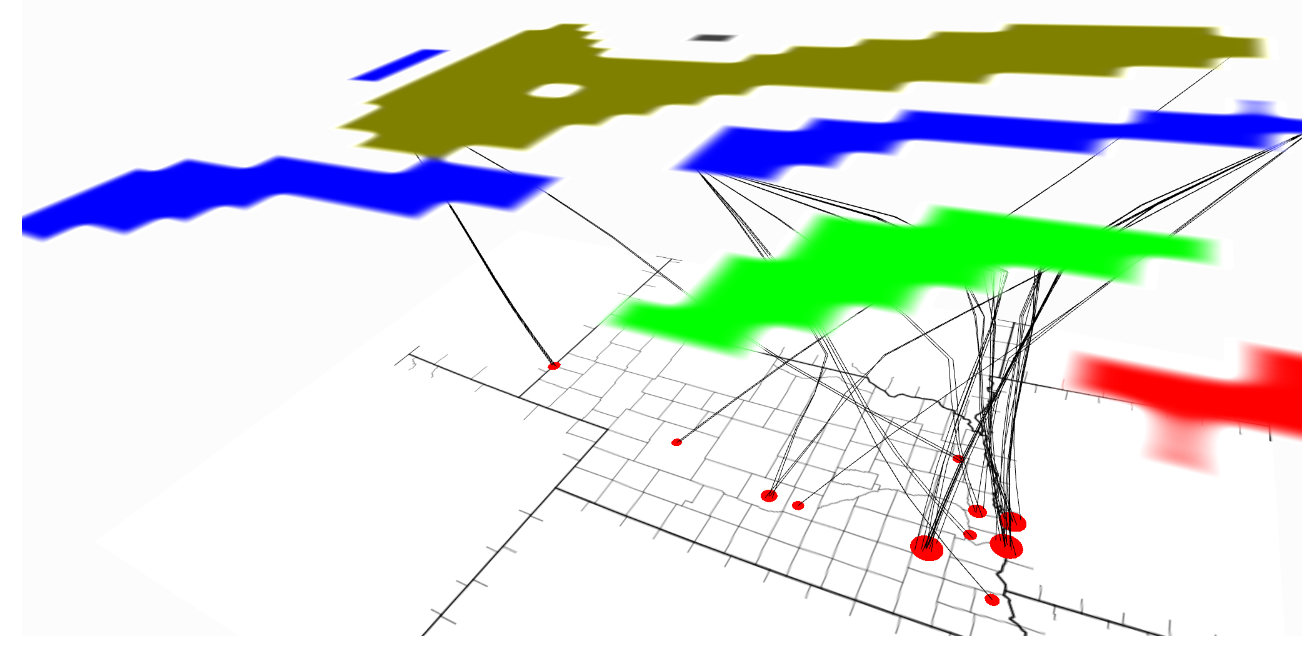
\includegraphics[scale=0.09]{blurBefore}}\quad
  \subfigure[After blurring]{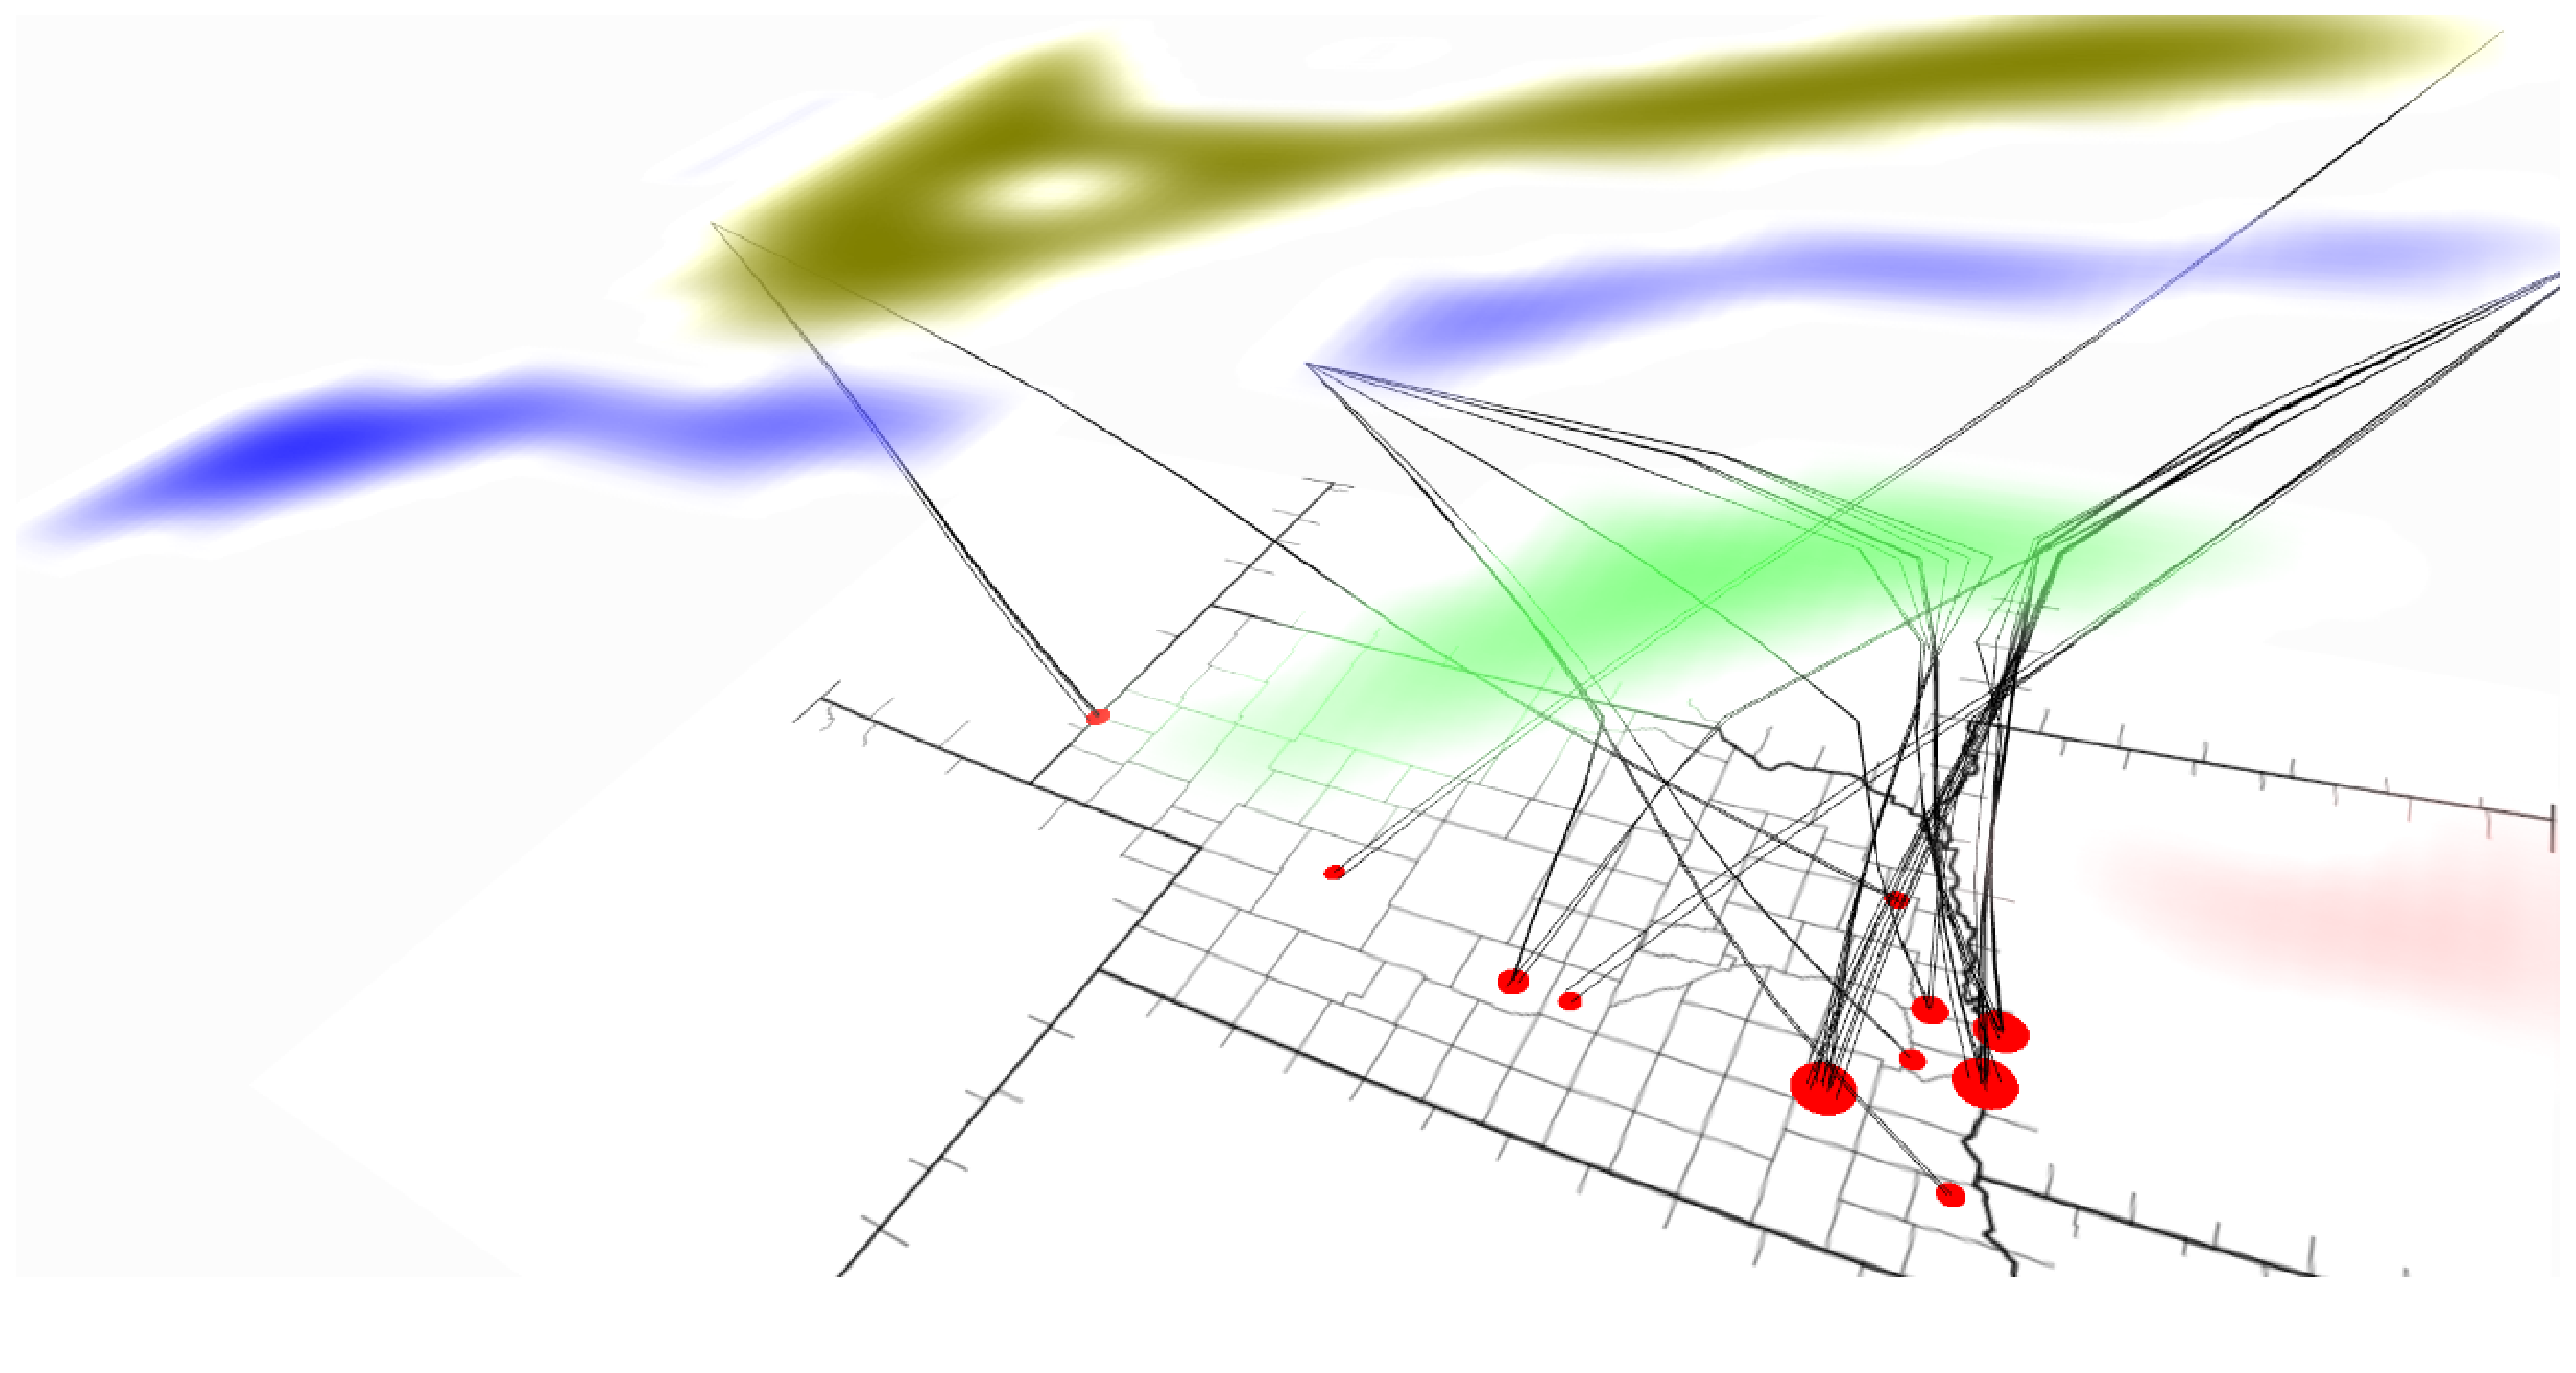
\includegraphics[scale=0.09]{blurAfter}}
\caption{Clustering of the weather. In this hour we see five different clusters. The blue cluster is seen in three different locations.}
\label{fig:blur}
\end{figure}

\begin{figure*}[htp]
  \centering
  \subfigure[Half good half bad]{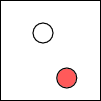
\includegraphics[scale=1.5]{sample}}\quad
  \subfigure[Half good half bad centers]{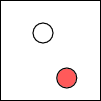
\includegraphics[scale=1.5]{sample}}\quad
  \subfigure[Corners]{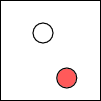
\includegraphics[scale=1.5]{sample}}
\caption{Determining the best position for indicating negative and positive tweets in the cloud clusters.}
\label{fig:corners}
\end{figure*}

\subsection{Line Bundling}
Each bundle is composed of multiple lines where each line represents one tweet. Every bundle represents positive or negative sentiment. The sentiment is represented in two ways. Depending on which corner the bundle is linked to indicates the sentiment, also the more intuitive notion is the color of the bundle. Naturally we associate the positive sentiments to the green bundles and the negative sentiments to the red bundles.

The opacity of each bundle represents the intensity of the correlation between the cluster and the tweets. The bolder the line the stronger the relationship between the two points is. The primary cluster has a stronger hue in comparison to the secondary and tertiary clusters. Both of these links will have a staggered decrease of intensity of color. Thus, we state that the more prominent the link between the tweet and the cluster the higher the opacity of the line.
